\documentclass{beamer}
\usepackage[utf8]{inputenc}

\usetheme{Madrid}
\usecolortheme{default}
\usepackage{amsmath,amssymb,amsfonts,amsthm}
\usepackage{txfonts}
\usepackage{tkz-euclide}
\usepackage{listings}
\usepackage{adjustbox}
\usepackage{array}
\usepackage{tabularx}
\usepackage{gvv}
\usepackage{lmodern}
\usepackage{circuitikz}
\usepackage{tikz}
\usepackage{graphicx}
\usepackage{gensymb} % For using \degree symbol
\usepackage{enumitem}

\setbeamertemplate{page number in head/foot}{} % This line removes the page counter


% Title Information
\title{5.3.37}
\date{October 11, 2025}
\author{ADHARVAN KSHATHRIYA BOMMAGANI - EE25BTECH11003}

\begin{document}

% Title Slide
\frame{\titlepage}

% Question Slide
\begin{frame}{Question}
Draw the graphs of the following equations
\begin{center}
    3x - 4y + 6 = 0 \\
    3x + y - 9 = 0
\end{center}
Also, determine the co-ordinates of the vertices of the triangle formed by these lines and the X-axis.
\end{frame}

% Step 1: Given Lines
\begin{frame}{Theoretical Solution}
The triangle is formed by the intersection of three lines:

    The two given lines.
    The X-axis, which has the equation $y=0$.

\bigskip
In vector normal form, the lines are:
\begin{align}
    L_1: \myvec{3 \\ -4}^\top \myvec{x \\ y} &= -6 \\
    L_2: \myvec{3 \\ 1}^\top \myvec{x \\ y} &= 9 \\
    L_3: \myvec{0 \\ 1}^\top \myvec{x \\ y} &= 0 \quad \text{(X-axis)}
\end{align}
The vertices, $\vec{A}$, $\vec{B}$, and $\vec{C}$, are the intersection points of these lines.
\end{frame}

% Step 2: Finding Vertex A
\begin{frame}{Theoretical Solution}
We solve the system: $3x - 4y = -6$ and $3x + y = 9$.
\bigskip
The augmented matrix is:
\begin{align}
    \myaugvec{2}{
        3 & -4 & -6 \\
        3 & 1 & 9
    }
    \xrightarrow{R_2 \to R_2 - R_1}
    \myaugvec{2}{
        3 & -4 & -6 \\
        0 & 5 & 15
    }
\end{align}
\begin{itemize}
    \item From $R_2$: $5y = 15 \implies y=3$.
    \item Substituting into $R_1$: $3x - 4(3) = -6 \implies 3x = 6 \implies x=2$.
\end{itemize}
\begin{align}
    \vec{A}=\myvec{2 \\ 3}
\end{align}
\end{frame}

% Step 3: Finding Vertex B
\begin{frame}{Theoretical Solution}
We solve the system: $3x - 4y = -6$ and $y = 0$.
\bigskip
Substituting $y=0$ into the first equation:
\begin{align}
    3x - 4(0) &= -6 \\
    3x &= -6 \\
    x &= -2
\end{align}
\bigskip
\begin{align}
    \vec{B}=\myvec{-2 \\ 0}
\end{align}
\end{frame}

% Step 4: Finding Vertex C
\begin{frame}{Theoretical Solution}
We solve the system: $3x + y = 9$ and $y = 0$.
\bigskip
Substituting $y=0$ into the first equation:
\begin{align}
    3x + 0 &= 9 \\
    3x &= 9 \\
    x &= 3
\end{align}
\bigskip
\begin{align}
    \vec{C}=\myvec{3 \\ 0}
\end{align}
\end{frame}

% Step 5: Final Answer
\begin{frame}{Theoretical Solution}
The coordinates of the vertices of the triangle are:
\begin{itemize}
    \item \textbf{Vertex A}: $(2, 3)$
    \item \textbf{Vertex B}: $(-2, 0)$
    \item \textbf{Vertex C}: $(3, 0)$
\end{itemize}
\end{frame}

% Step 6: Figure
\begin{frame}{Plot}
\centering
\begin{figure}[h!]
    \centering
    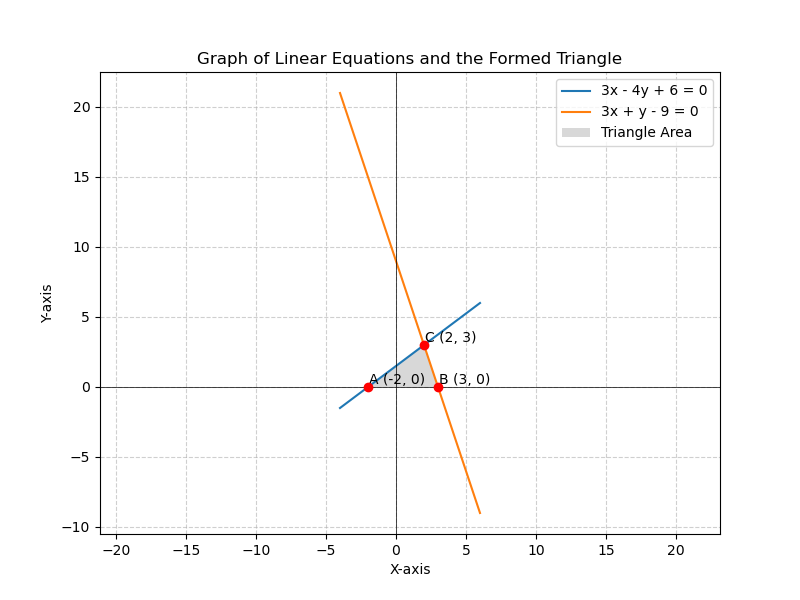
\includegraphics[width=0.8\columnwidth]{figs/fig1.png}
    \caption{figure for 5.3.37}
\end{figure}
\end{frame}

\end{document}